\documentclass{beamer}
\usepackage{amsmath}
\usepackage[english]{babel} %set language; note: after changing this, you need to delete all auxiliary files to recompile
\usepackage[utf8]{inputenc} %define file encoding; latin1 is the other often used option
\usepackage{csquotes} % provides context sensitive quotation facilities
\usepackage{graphicx} %allows for inserting figures
\usepackage{booktabs} % for table formatting without vertical lines
\usepackage{textcomp} % allow for example using the Euro sign with \texteuro
\usepackage{stackengine}
\usepackage{wasysym}
\usepackage{tikzsymbols}
\usepackage{textcomp}
% ELIMINAR COMANDOS DE NAVEGACION%%%%%%%%%%%
\setbeamertemplate{navigation symbols}

%\newcommand{\bubblethis}[2]{
 %       \tikz[remember picture,baseline]{\node[anchor=base,inner sep=0,outer sep=0]%
 %       (#1) {\underline{#1}};\node[overlay,cloud callout,callout relative pointer={(0.2cm,-0.7cm)},%
 %       aspect=2.5,fill=yellow!90] at ($(#1.north)+(-0.5cm,1.6cm)$) {#2};}%
 %   }%
%\tikzset{face/.style={shape=circle,minimum size=4ex,shading=radial,outer sep=0pt,
 %       inner color=white!50!yellow,outer color= yellow!70!orange}}

%% Some commands to make the code easier
\newcommand{\emoticon}[1][]{%
  \node[face,#1] (emoticon) {};
  %% The eyes are fixed.
  \draw[fill=white] (-1ex,0ex) ..controls (-0.5ex,0.2ex)and(0.5ex,0.2ex)..
        (1ex,0.0ex) ..controls ( 1.5ex,1.5ex)and( 0.2ex,1.7ex)..
        (0ex,0.4ex) ..controls (-0.2ex,1.7ex)and(-1.5ex,1.5ex)..
        (-1ex,0ex)--cycle;}
\newcommand{\pupils}{
  %% standard pupils
  \fill[shift={(0.5ex,0.5ex)},rotate=80] 
       (0,0) ellipse (0.3ex and 0.15ex);
  \fill[shift={(-0.5ex,0.5ex)},rotate=100] 
       (0,0) ellipse (0.3ex and 0.15ex);}

\newcommand{\emoticonname}[1]{
  \node[below=1ex of emoticon,font=\footnotesize,
        minimum width=4cm]{#1};}
\usepackage{scalerel}
\usetikzlibrary{positioning}
\usepackage{xcolor,amssymb}
\newcommand\dangersignb[1][2ex]{%
  \scaleto{\stackengine{0.3pt}{\scalebox{1.1}[.9]{%
  \color{red}$\blacktriangle$}}{\tiny\bfseries !}{O}{c}{F}{F}{L}}{#1}%
}
\newcommand\dangersignw[1][2ex]{%
  \scaleto{\stackengine{0.3pt}{\scalebox{1.1}[.9]{%
  \color{red}$\blacktriangle$}}{\color{white}\tiny\bfseries !}{O}{c}{F}{F}{L}}{#1}%
}
\usepackage{fontawesome} % Social Icons
\usepackage{epstopdf} % allow embedding eps-figures
\usepackage{tikz} % allows drawing figures
\usepackage{amsmath,amssymb,amsthm} %advanced math facilities
\usepackage{lmodern} %uses font that support italic and bold at the same time

\usepackage{tikz}
\usepackage{tcolorbox}


\usefonttheme[onlymath]{serif} %set math font to serif ones

\definecolor{beamerblue}{rgb}{0.2,0.2,0.7} %define beamerblue color for later use

%%% defines highlight command to set text blue
\newcommand{\highlight}[1]{{\color{blue}{#1}}}


%%%%%%% commands defining backup slides so that frame numbering is correct

\newcommand{\backupbegin}{
   \newcounter{framenumberappendix}
   \setcounter{framenumberappendix}{\value{framenumber}}
}
\newcommand{\backupend}{
   \addtocounter{framenumberappendix}{-\value{framenumber}}
   \addtocounter{framenumber}{\value{framenumberappendix}}
}

%%%% end of defining backup slides

%Specify figure caption, see also http://tex.stackexchange.com/questions/155738/caption-package-not-working-with-beamer
\setbeamertemplate{caption}{\insertcaption} %redefines caption to remove label "Figure".
%\setbeamerfont{caption}{size=\scriptsize,shape=\itshape,series=\bfseries} %sets figure  caption bold and italic and makes it smaller

\newtcolorbox{boxA}{
    fontupper = \bf,
    boxrule = 1.5pt,
    colframe = black % frame color
}

\usetheme{Boadilla}

\usepackage{hyperref}

% --------------------
% Overall information
% --------------------
\title[Economía I]{Economía I \vspace{4mm}
\\ Magistral 9: Instituciones}
\date{}
\author[Riottini]{Franco Riottini}
\vspace{0.4cm}
\institute[]{Universidad de San Andrés} 


\begin{document}

\begin{frame}
\titlepage
\centering

\includegraphics[scale=0.2]{../Figures/logoUDESA.jpg} 
\end{frame}


\begin{frame}
\frametitle{Cuál es la diferencia...}
\centering
\includegraphics[scale=0.4]{../Figures/Mina.png}
\end{frame}

\begin{frame}
\frametitle{Cuál es la diferencia...}
\begin{itemize}
    \item Durante el 2023, el sector minero argentino alcanzó aproximadamente US\$4.500 millones de exportaciones y empleó formalmente a 90 mil personas.
    \item En cambio, Chile que exportó US\$60.000 millones y empleó más de 920 mil personas!!
    \item Argentina es parte de la región más grande del continente americano con depósitos minerales metálicos. Pachón es una de las 10 mayores reservas de cobre del mundo. Se conoce desde 1964 pero todavía no se pudo poner en marcha.
    \item Los Pelambres (Chile) funciona desde 1999 y en 2022 generó más de U\$S 3000 millones.
\end{itemize}
\end{frame}

\begin{frame}
\centering
“Una de las conclusiones más interesantes del neoinstitucionalismo económico es que la política y la economía están inextricablemente relacionadas y que no podemos explicar el desempeño económico de una determinada sociedad sin considerar esta relación.” Douglas C. North
\end{frame}

\begin{frame}{Asignaciones e instituciones}
    \begin{itemize}
        \item En esta clase vamos a estudiar como las instituciones afectan los resultados económicos.
        \item Una asignación es el resultado de una interacción económica, pero está determinada por distintos factores:
        \begin{itemize}
            \item La tecnología y los recursos naturales determinan lo posible.
            \item Las instituciones dificultan o facilitan el accionar de los agentes\dots
        \end{itemize}
        \item Generalmente, nos interesan dos aspectos sobre las instituciones:
        \begin{itemize}
            \item Queremos describirlas: ¿Como afecta la asignaciones?
            \item Queremos evaluarlas: ¿Cuales son las mejores instituciones?
        \end{itemize}
    \end{itemize} 
\end{frame}

\begin{frame}
\frametitle{¿Qué es una institución?}
De acuerdo a North son las reglas del juego en una sociedad que reducen la incertidumbre y proveen un marco para la interacción social
    \begin{itemize}
        \item Reducen los costos de transacción, proporcionando una estructura a la vida cotidiana.
        \item Definen y limitan el conjunto de opciones de los individuos.
        \item Son creadas por seres humanos.
        \item Normas formales e informales.
        \item Afectan la performance de la economía.
        \item Pueden inducir a aumentar o reducir la productividad.
    \end{itemize}
\end{frame}

\begin{frame}
\frametitle{Formales o informales}
\centering
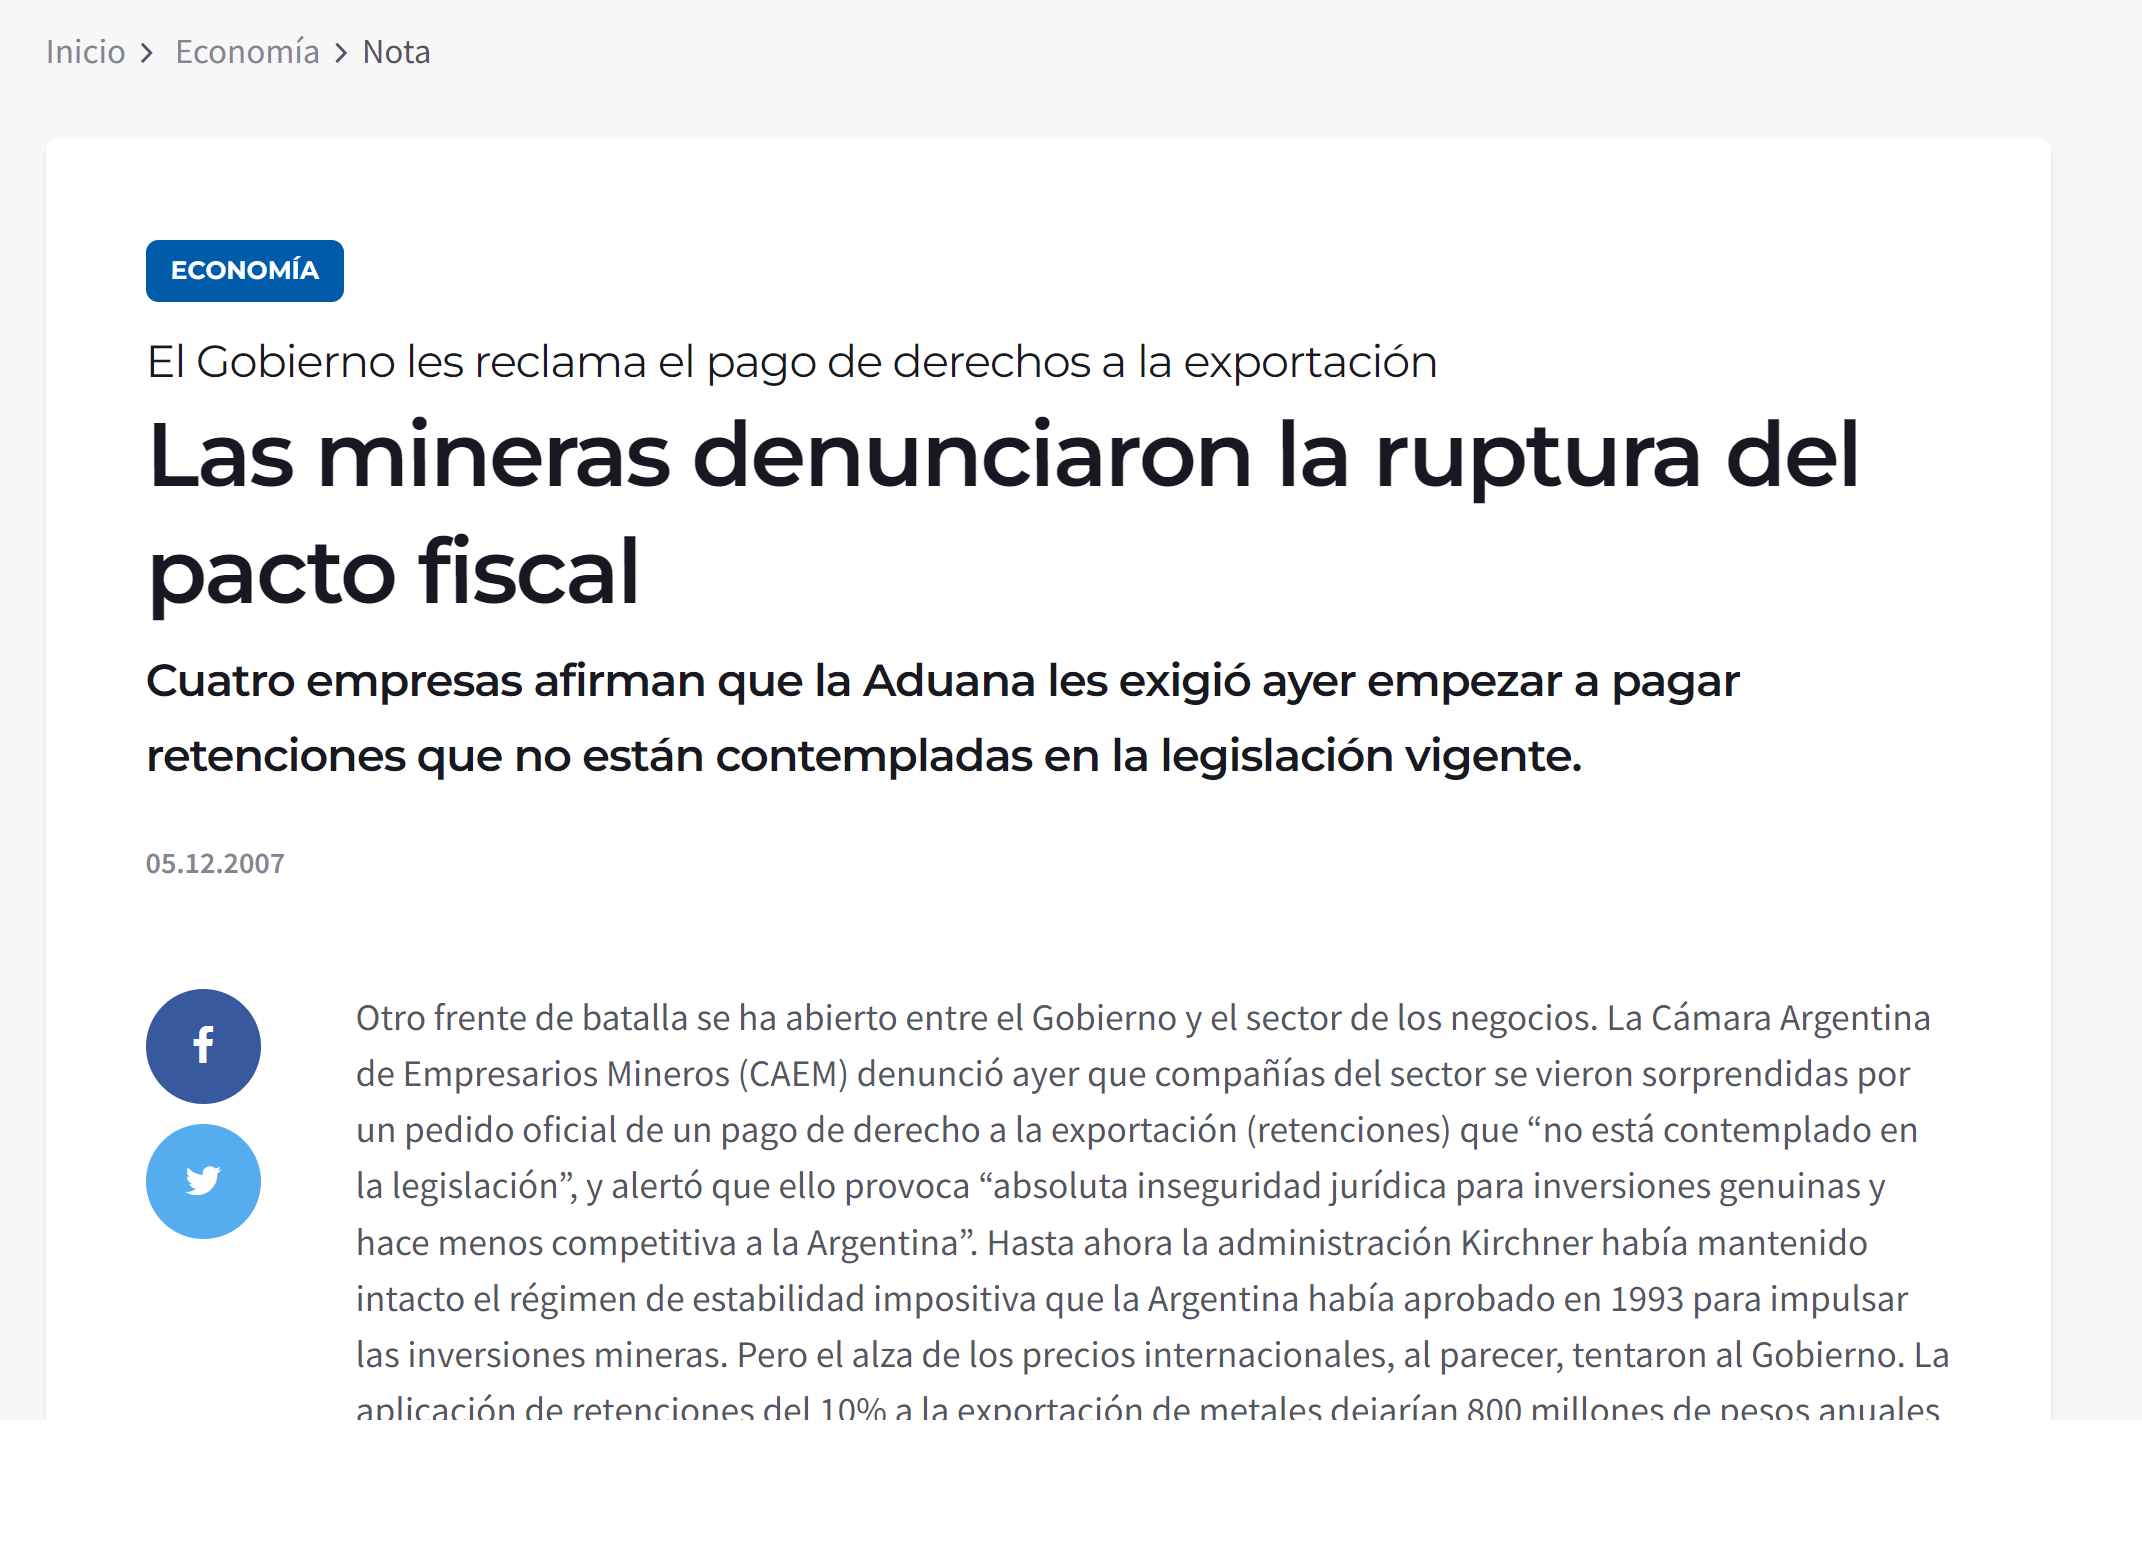
\includegraphics[scale=0.4]{../Figures/Mina2.png}
\end{frame}


\begin{frame}{¿Qué es una institución?}
    Greif [2006] dio una definición más precisa:
        \begin{boxA}
            \centering
            ``Una institución es un sistema de reglas, creencias, normas y organizaciones que juntas generan una regularidad en la conducta''\vspace{2mm}
        \end{boxA}
    Una regularidad en el comportamiento social 
        \begin{itemize}
            \item Comportamiento en situaciones recurrentes...
            \item ... llevado a cabo por individuos que ocupan una posición social particular.\vspace{2mm}
        \end{itemize}
    Cada componente del sistema
        \begin{itemize}
            \item Es social al ser hecho por el hombre...
            \item ... y exógeno a cada individuo cuyo comportamiento influye
        \end{itemize}
\end{frame}

\begin{frame}
\frametitle{Los componentes del sistema}
\begin{itemize}
    \item Las reglas, cuando son reconocidas socialmente, guían el comportamiento
    \begin{itemize}
        \item Crean un conocimiento compartido.
        \item Proveen información y coordinan el comportamiento.
        \item Indican el comportamiento socialmente aceptable.
    \end{itemize}
    \item Las creencias y normas motivan a seguir reglas
    \begin{itemize}
        \item Normas y creencias internalizadas.
    \end{itemize}
    \item Las organizaciones (formales o informales)
    \begin{itemize}
        \item Producen y difunden reglas.
        \item Perpetúan creencias y normas.
        \item Influyen en el conjunto de creencias factibles.
    \end{itemize}
\end{itemize}
\end{frame}

\begin{frame}
\frametitle{Discutamos ejemplos...}
\centering
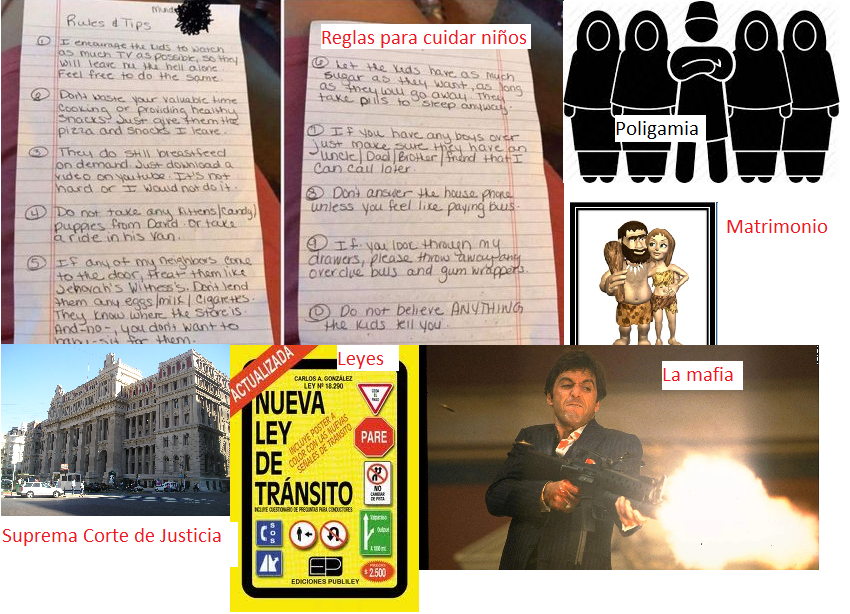
\includegraphics[scale=0.45]{../Figures/Tema_04.1_examples.png}
\end{frame}

\begin{frame}
\frametitle{Importancia de las instituciones}
\begin{itemize}
    \item Al generar una regularidad en la conducta, las instituciones determinan qué tan grandes son los costos de transacción, y quien los paga
    \begin{itemize}
        \item Esto afecta si los agentes actúan o no.
        \item Buenas instituciones reducen los costos de transacción, lo que implica más transacciones económicas.
    \end{itemize}
    \item ¿Importan para el crecimiento?
    

    \begin{center}
        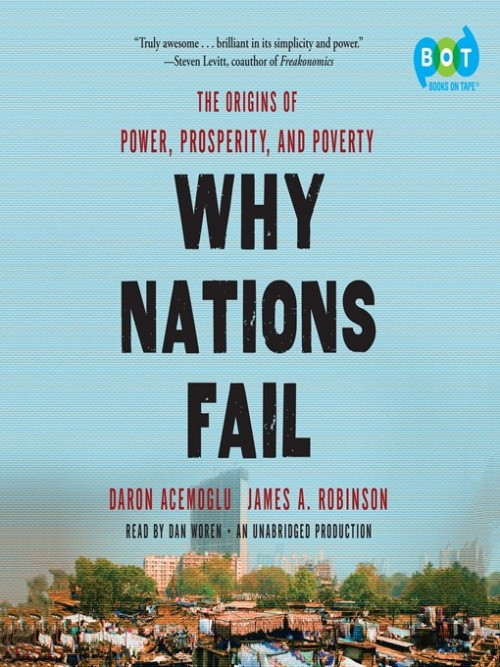
\includegraphics[scale=0.2]{../Figures/Why-Nations-Fail.jpg}
    \end{center}
\end{itemize}
\end{frame}

\begin{frame}{Instituciones y eficiencia}
    \begin{itemize}
        \item Las instituciones afectan que tan eficiente (en el sentido de Pareto) son las asignaciones.
        \item Intituciones adecuadas nos pueden ayudar a alcanzar un equilibrio eficiente mientras que las ineficientes.
        \item Sin embargo, lo económico no necesariamente es el único objetivo de las instituciones.
        \item Conocer los criterios bajo los cuales una asignaión es justa o injusta es un problema de larga tradicion en filosofía y derecho.
    \end{itemize}
\end{frame}

\begin{frame}
\frametitle{Asignaciones y justicia}
\begin{itemize}
    \item Una asignación puede ser considerada justa o injusta en sí
    \begin{itemize}
        \item Un juicio substantivo de la justicia:
        \begin{itemize}
            \item Necesitamos una métrica de "lo que nos parece bien o mal"
            \item ¿Qué define que es justo?
        \end{itemize}
    \end{itemize}
    \item  Una asignación puede ser considerada justo o  injusta por la forma en que se llegó a ese resultado\vspace{2mm}
    \begin{itemize}
        \item Un juicio procedimental de la justicia
        \begin{itemize} 
            \item Necesitamos entender las reglas de juego y cómo se llegó al resultado \\
            \item ¿Fueron los intercambios voluntarios?, ¿Fueron algunos individuos discriminados?, etc.
        \end{itemize}
    \end{itemize}
\end{itemize}
\end{frame}

\begin{frame}{Economía y justicia}
    \begin{itemize}
        \item Los valores que tiene la gente sobre lo que es justo y lo que no, varía entre individuos. ¿Podemos construir una teoría de la moral?
        \item El filósofo americano John Rawls sugirió como hacerlo:
        \begin{itemize}
            \item El velo de la ignorancia: Imaginarse detrás del velo de la ignorancia, es decir, imaginarse un tema sin saber que lugar ocuparemos en esa sociedad.
            \item Elaboramos un juicio o evaluamos una institución desde atrás de ese velo.
        \end{itemize}
        \item Por ejemplo: ¿los ricos deberían pagar más impuestos? ¿las personas con habilidades especiales deberían recibir una compensación del resto de la sociedad? 
    \end{itemize}
\end{frame}

\begin{frame}{Economía y justicia}
    \begin{itemize}
        \item La economía no hace juicios sobre lo que es justo o no pero sí puede ayudarnos a pensar una serie de cosas:
        \begin{itemize}
            \item Cómo las instituciones (reglas del juego) afectan las asignaciones y la desigualdad.
            \item Cómo explotar todas las situaciones de win-win que no generan conflicto.
            \item Qué tipo de políticas públicas son las mejores para lidiar con la injusticia.
        \end{itemize}
    \end{itemize}
\end{frame}


\begin{frame}{Entendiendo el valor de las instituciones}
    Arrancamos con una frontera de posibilidades de producción.
    \begin{itemize}
    \item La frontera factible nos indica lo que es tecnológicamente posible.
    \item Pero ahora vamos a sumar una restricción que considera lo que es biológicamente posible.
        \begin{itemize}
            \item ¿Qué significa esto?
            \begin{itemize}
                \item Hay un mínimo de recursos que el individuo necesita para sobrevivir, aún si no produce nada...
                \item ... y cuantas mas energías utiliza produciendo, más recursos va a necesitar
            \end{itemize}
        \end{itemize}
    \end{itemize}
\end{frame}

\begin{frame}{La restricción biológica}
    \centering
    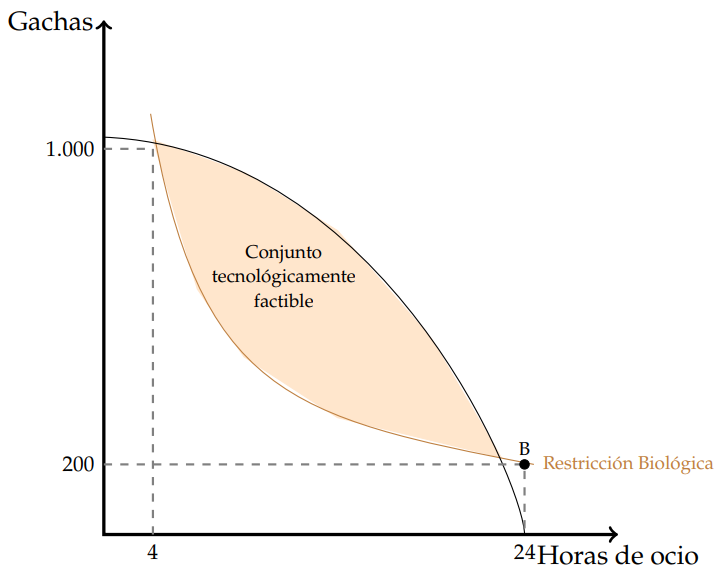
\includegraphics[scale=0.6]{../Figures/C19.6.png}
\end{frame}


\begin{frame}{El objetivo es comparar distintas instituciones}
    Comparamos escenarios donde:
        \begin{itemize}
            \item Situaciones históricas
            \begin{itemize}
                \item El régimen de esclavitud (Imperio Romano)
                \item Campesinos libres (EEUU en el siglo XVIII)
                \item Servidumbre con renta fija (Medioevo)
                \item Servidumbre con renta variable (Medioevo)
                \item La China comunista
                \item Un país con sindicatos
            \end{itemize}
        \end{itemize}
    ¿En qué forma queremos compararlas? Por ahora, en términos de eficiencia de Pareto
\end{frame}

\begin{frame}{¿Qué punto elige el amo?}
    \centering
    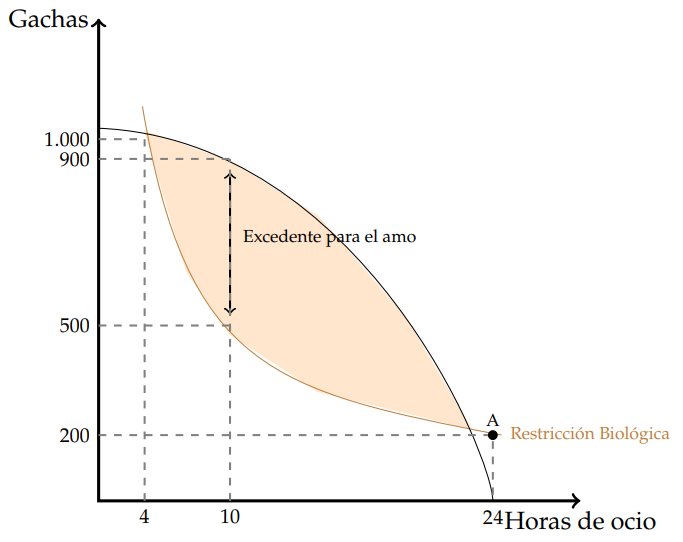
\includegraphics[scale=0.6]{../Figures/C19.7.png}
\end{frame}


\begin{frame}{El equilibrio de la esclavitud}
    \centering
    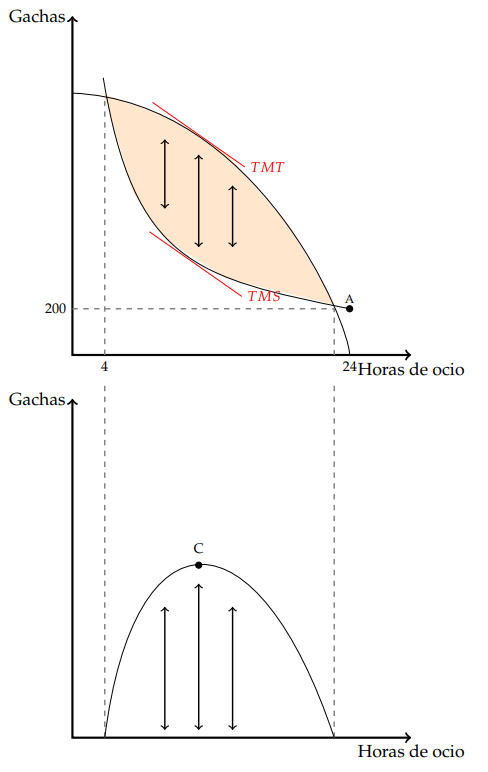
\includegraphics[scale=0.5]{../Figures/C19.8.png}
\end{frame}

\begin{frame}{Ahora el esclavo se libera!}
    \begin{center}
        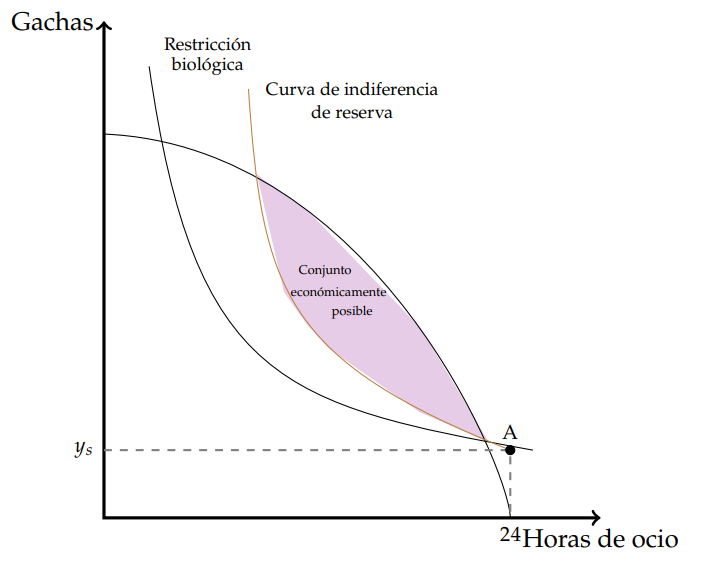
\includegraphics[scale=0.5]{../Figures/C19.9.png}   
    \end{center}
    \begin{itemize}
        \item Ahora el campesino toma en cuenta la desutilidad del trabajo. Puede decidir no hacerlo.
        \item Toma en cuenta el costo de oportunidad. El trabajador tiene otros ingresos u opciones que le garantizan la supervivencia.
    \end{itemize}
\end{frame}


\begin{frame}
\frametitle{La decisión del campesino libre}
\begin{center}
    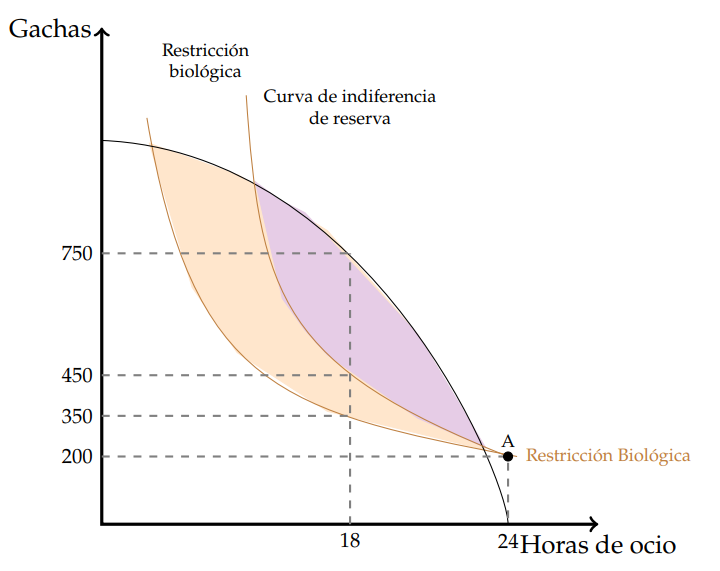
\includegraphics[scale=0.6]{../Figures/C19.10.png}   
\end{center}
\end{frame}

\begin{frame}{Las diferencias entre la esclavitud y la libertad}
    \centering
    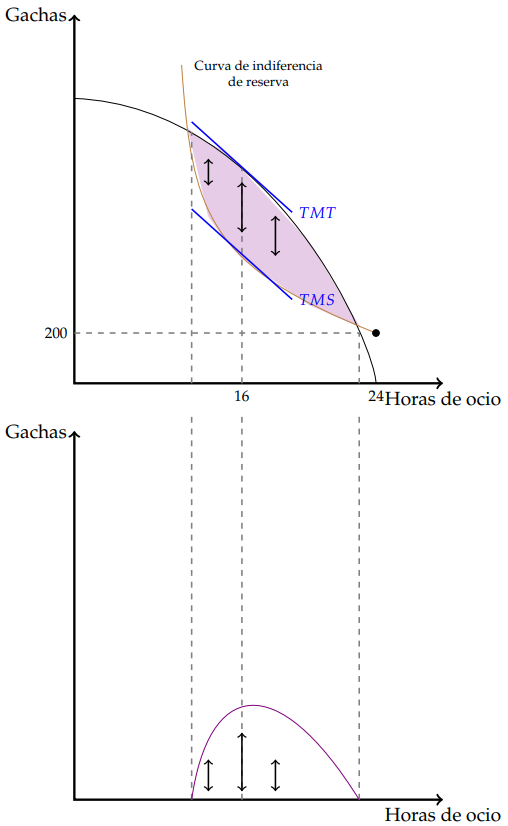
\includegraphics[scale=0.5]{../Figures/C19.11.png}
\end{frame}


\begin{frame}{Las diferencias entre la esclavitud y la libertad}
    \begin{itemize}
        \begin{boxA}
            \centering
            En el óptimo, el trabajador elegirá el nivel de trabajo donde el costo marginal iguala a la producción marginal, que es el punto en el que se maximiza la diferencia entre estas dos curvas.
        \end{boxA}
        \item El punto máximo es cuando se iguala la pendiente de la curva de transformación con la de la curva de indiferencia de reserva. 
        \item El dueño de la tierra trabaja menos que en el régimen de esclavitud.
        \item Pero eso es óptimo: porque el régimen de esclavitud no tomaba en cuenta su desutilidad!
        \item El cambio de instituciones cambió la asignación (y la distribución).
    \end{itemize}
\end{frame}

\begin{frame}
\frametitle{Servidumbre medieval: servidumbre fija}
\begin{itemize}
    \item Estamos en la edad media donde un señor feudal es dueño de la tierra. 
    \item Se le permite a un campesino trabajar la tierra pero a cambio de una "servidumbre". 
    \item  En este caso asumimos que el pago es un monto fijo de producción 
    \item Reduce lo que se lleva el campesino desplazando su retorno hacia abajo.
    \item La producción no se modifica pero sí su distribución (ahora el campesino tiene que pasarle parte al señor feudal). 
\end{itemize}
\end{frame}

\begin{frame}{Servidumbre medieval: servidumbre fija}
    \centering
    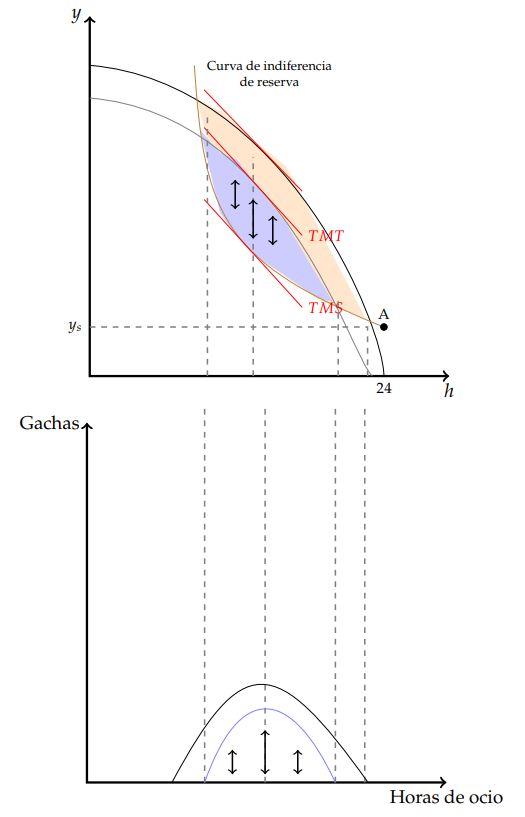
\includegraphics[scale=0.45]{../Figures/C19.12.png}
\end{frame}

\begin{frame}{Servidumbre medieval: un porcentaje de la producción}
    \begin{itemize}
        \item Ahora asumimos que el pago es un porcentaje de la producción 
        \item Reduce lo que se lleva el campesino desplazando su retorno hacia abajo pero no de manera paralela sino que lo que se reduce crece con la producción
        \item La producción ahora cae respecto al caso anterior
        \item Hay una distorsión en la producción pero el riesgo está mejor distribuido entre productor y señor feudal. 
    \end{itemize}
\end{frame}

\begin{frame}
\frametitle{Servidumbre medieval: un porcentaje de la producción}
\centering
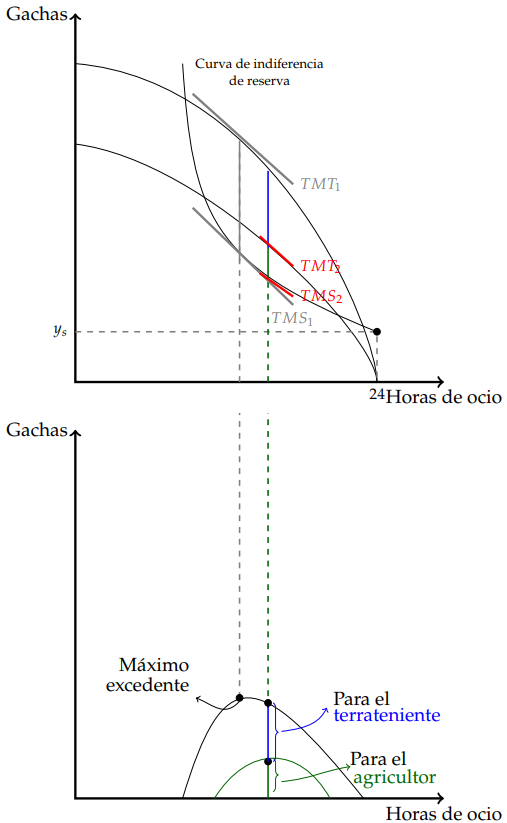
\includegraphics[scale=0.45]{../Figures/C19.13.png}
\end{frame}

\begin{frame}{Diversificando riesgo en la Edad Media}
    \centering
    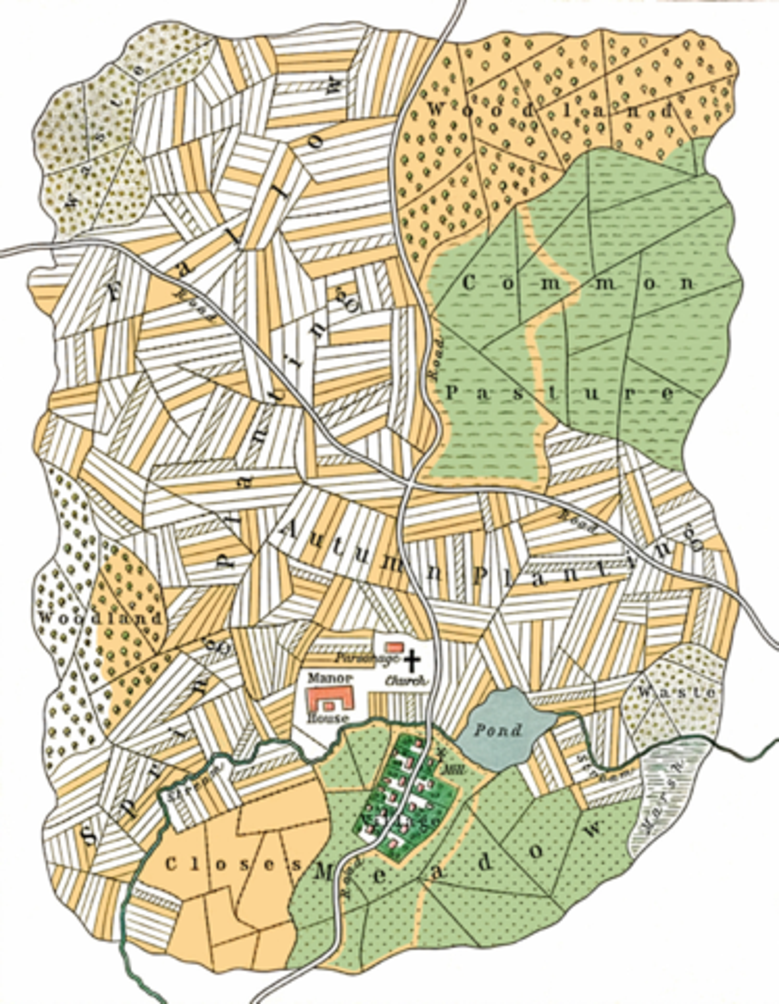
\includegraphics[scale=0.4]{../PastedGraphic-1.pdf}
    \begin{itemize}
        \item Una manera de acotar el riesgo era partiendo las parcelas y distribuyéndolas en un área geográfica más amplia. 
    \end{itemize}
\end{frame}

\begin{frame}{La China de Mao}
    \begin{center}
        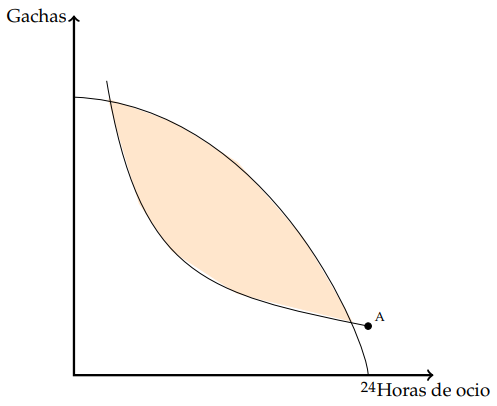
\includegraphics[scale=0.6]{../Figures/C19.15.png}
    \end{center}
    \begin{itemize}
        \item Si siempre recibo lo mismo, sin importar la cantidad que trabajo, el óptimo está en el punto A donde el ocio es pleno y la producción es 0... 
    \end{itemize}
\end{frame}

\begin{frame}
\frametitle{La China de Mao }
\begin{itemize}
    \item Cuando Mao llega al poder decide la colectivización de las granjas
    \item Lo que recibe cada productor es independiente de lo que produce. 
    
    \item El productor maximiza su utilidad minimizando su trabajo 
     \item La producción baja a cero.  
     \item 40 millones de personas murieron de hambre
     \item ¡Vaya si las instituciones importan! 
\end{itemize}

\end{frame}

\begin{frame}
\frametitle{¿Qué pasa si hay un salario mínimo o un bono obligatorio?}
\centering

\includegraphics[scale=0.33]{../Figures/InstitucionesBono.png}
\end{frame}

\begin{frame}
\frametitle{¿Qué pasa si hay un salario mínimo o un bono obligatorio?}
\centering
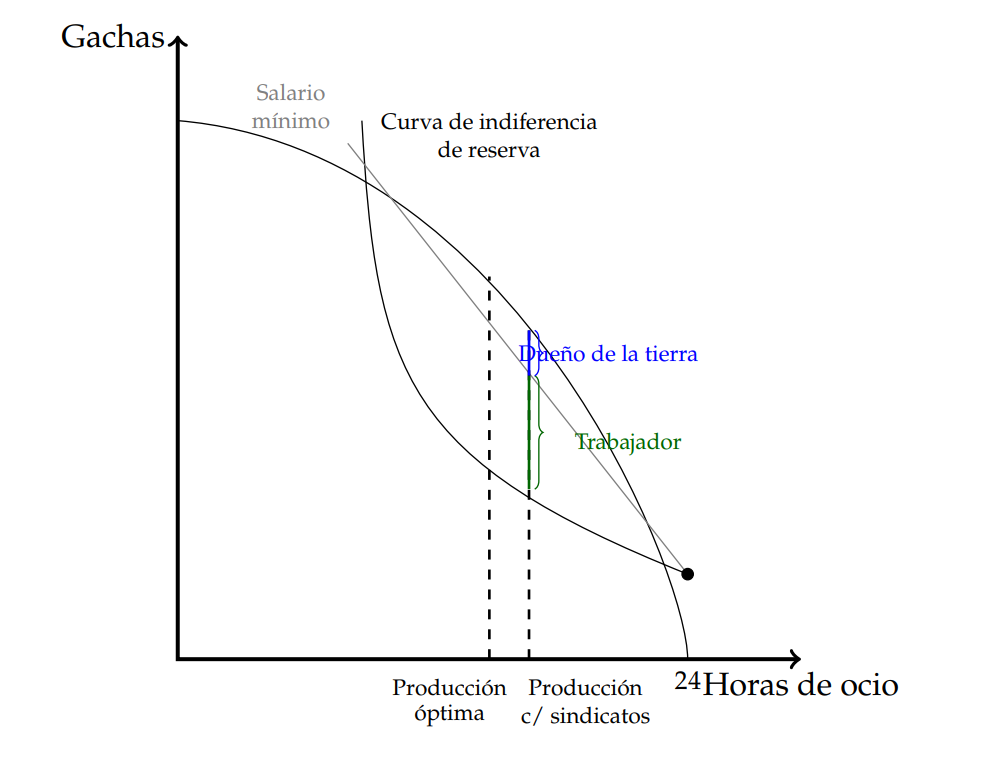
\includegraphics[scale=0.8]{../Figures/Salariominimo.png}
\end{frame}

\begin{frame}
\frametitle{El gobierno sindical de Sudáfrica}
\begin{itemize}
    \item La remuneración de los trabajadores la define un "sindicato". 
    \item  Asumimos esa remuneración es mayor a la que ocurriría naturalmente
    \item Definido el salario el dueño de la tierra define cuanto producir
    \item  La producción cae, pero la parte de la torta que se lleva el trabajador puede subir. 
\end{itemize}
\end{frame}

\end{document}
